\documentclass[a4paper, 11pt]{exam}
\usepackage{titling}
\newcommand{\subtitle}[1]{%
  \posttitle{%
    \par\end{center}
    \begin{center}\large#1\end{center}
    }%
}

\usepackage{url}
\usepackage{amsmath,amsthm,enumitem,amssymb}
\usepackage{graphicx}
\usepackage{hyperref}
\usepackage{float}
\renewcommand{\labelenumii}{\roman{enumii}}

\title{Homework Assignment 2}
\subtitle{CS/ECE 6810: Computer Architecture \\
Jan 31,2018\\
Marek Baranowski}

\author{ \\
\textbf{Pipelining}}
\date{Due Date: Feb 13, 2018.\\
90 points}

\begin{document}
\maketitle
\begin{center}
\fbox{\fbox{\parbox{5.9in}{\centering
Important Notes:
\begin{itemize}
\item Solutions turned in must be your own. Please, mention references (if any) at the end of each question. Please refrain from cheating.
\item All solutions must be accompanied by the equations used/logic/intermediate steps. Writing only the final answer will receive \textbf{zero} credit.
\item All units must be mentioned wherever required.
\item Late submissions \textbf{(after 11:59 pm on 02/13/2018)} will not be accepted
\item All submissions must be in PDF only. Scanned copies of handwritten solutions will not be accepted as a valid submission.
\end{itemize}
}}}
\end{center}
\vspace{0.2in}

\begin{enumerate}
	\item \textbf {Pipelining Performance}
    Consider a single-cycle processor in which the execution of
every instruction completes in 10 ns. The goal is to execute a user application that consists of 1000 instructions.
	\begin{enumerate}
    \item If the single cycle processor can execute one instruction per cycle, find the CPU time. \textbf{(5 points)}
    
\fbox{\parbox{5.5in}{
    \textbf{Answer}
    The execution time is
    
     $CI\cdot CT \cdot CPI = 1000\cdot10ns\cdot1=10\mu$s
    }}
    \newline
    
   
    \item Assuming a 1ns additional delay for pipeline registers and perfect circuit partitioning and pipelining, find the speedup gained by making the processor 10-stage pipelined. Assume that 2 bubbles (NOPs) are necessary every 10 cycles for load and branch instructions. \textbf{(15 points)}
    
\fbox{\parbox{5.5in}{
The CPI for this program on this architecture is $\frac{12}{10}=1.2$. CT=1ns+1ns=2ns since each stage is 1ns and there is a 1ns delay ($CT_{new} = (t+{CT\over P}$).
To get the speed up we calculate:
\begin{align*}
\frac{Time_{old}}{Time_{new}} =
\frac{CI\cdot (CT+t) \cdot CPI}{1000\cdot2\text{ns}\cdot1.2} = 
\frac{11\mu\text{s}}{2.4\mu\text{s}} = 4.58.
\end{align*}
    }}
	\newline
    
	\end{enumerate}
    
    \item \textbf{Control Hazards} Consider an in-order five-stage pipeline that determines the branch
target by the end of the 3rd pipeline stage (i.e., the execute stage). To avoid branch related stalls, the instruction set architecture (ISA) defines two branch delay slots. Assume that (a) all stalls in the processor are branch-related, (b) $20\%$ of all instructions are branches, (c) a branch is taken $60\%$ of the time, and (d) you could move two instructions from the taken side into the branch delay slot. What is the expected CPI for
this processor? \textbf{(15 points)} 

\fbox{\parbox{5.8in}{
    \textbf{Answer}
When a branch is taken, the CPI will be 1 since the work will have been completed in the filled branch-delay slots. If a branch is not taken, then two useless instructions will have to be canceled: this means we effectively complete 5 instructions in 7 cycles for a CPI of $\frac{7}{5}$.

To get the expected CPI we calculate:
\begin{align*}
CPI=0.6\cdot1+0.4\cdot\frac{7}{5}=1.16
\end{align*}
    }}
	\newline
    
	\item \textbf{Multi-cycle Instructions} A pipelined architecture comprises instruction fetch (IF), instruction issue (IS), register read (RR), execute (EX), and write-back (WB) stages. Except EX, each stage requires one clock cycle to complete. The EX stage includes 4
functional units, each of which can perform a floating-point operation —e.g., ADD, SUB, MULT, DIV, load, and store. The table below shows the latency of the operations in terms of the number of clock cycles. The pipeline implements all necessary forwarding paths for the ALU operations.

\begin{center}
\begin{tabular}{ |c|c|c|c|c|c|c| } 
 \hline
  & ADD & SUB & MULT & DIV & Load & Store \\ 
  \hline
 Latency & 1 & 1 & 3 & 4 & 1 & 1 \\ 
 \hline
\end{tabular}
\end{center}

\begin{enumerate}
\item Create a timing diagram for the following code showing the execution of the code in time (clock cycles). \textbf{(15 points)}

\fbox{\parbox{5.5in}{
    \textbf{Answer}
    \begin{figure}[H]
  \centering
    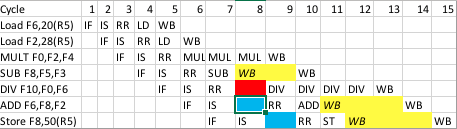
\includegraphics[width=.8\textwidth]{timeline.png}
    \caption{Red cells indicate stalls that are needed for data to be ready, yellow cells indicate delays for WB to maintain program order. \textit{WB} indicates where a write back could happen out of program order. Blue cells are a structural hazards.}
\end{figure}
    }}
	\newline

\item Identify all structural and data hazards in the following code. \textbf {(20 points)}

\fbox{\parbox{5.5in}{
    \textbf{Answer}
Read after write
\begin{itemize}
\item DIV needs F0 from MUL, but MUL won't complete in time.
\item MUL needs F2 from the second load, but I assume the ALU has perfect forwarding so is able to avoid the hazard.
\item SUB needs F6 from the first load, but Load finishes WB before SUB's RR so no forwarding is necessary to avoid the hazard. This is similar for DIV's dependence on F6.
\item ADD needs F2 from the second Load, but that is complete before ADD starts. ADD also starts two cycles (NOP before DIV) after SUB so F8 is ready for ADD.
\item Store depends on SUB's output, but SUB will have the value ready before ST executes.
\end{itemize}
Structural hazards\begin{itemize}
\item SUB, ADD and Store have a potential hazards in that they can write back before previous instructions perform a write-back. 
\item The DIV instruction causes a hazard for RR without adding NOP before it (seen as blue in the timeline).
\end{itemize}
    }}
	\newline

\begin {center}
Load F6, 20(R5) 

Load F2, 28(R5)

MUL F0, F2, F4

SUB F8, F6, F3

DIV F10, F0, F6

ADD F6, F8, F2

Store F8, 50(R5)

\end {center}

\end{enumerate}

\item \textbf{Points of Production and Consumption} n. Consider an un-pipelined processor where it takes 36 ns to go through the circuits and 0.5 ns for the latch overhead. Assume that the point of production and point of consumption in the unpipelined processor are separated by 12 ns. Assume that half the instructions do not introduce a data hazard and half the
instructions depend on their preceding instruction

\begin{enumerate}
\item What is the throughput of the processor with the un-pipelined architecture \textbf{(10 points)}

\fbox{\parbox{5.5in}{
    \textbf{Answer}
Since there is no pipeline, we will not have a data hazard, meaning no instruction will have to wait. In the un-pipelined architecture only one instruction is in the processor and it takes 36.5 ns to complete (including the latch delay). This gives a throughput of $\frac{1 instruction}{36.5ns} = 27.4$ million instructions/s.
 }}
	\newline
\item What is the throughput of the processor with a 12-stage pipeline? \textbf {(10 points)}

\fbox{\parbox{5.5in}{
    \textbf{Answer}
If we had perfect, 12-stage pipelining, each stage would take 3ns, plus the additional latch delay we get 3.5ns per cycle. In the original processor, there was a 12ns delay between the point of production and the point of consumption, corresponding to 4 pipe-line stages in the new processor.

With the assumption that half the instructions do not introduce data hazards, and the other half do, we effectively complete 2 instructions every 5 cycles because one of the stalls could be filled by a non-hazard instruction. This means we have a throughput of 
\begin{align*}
\frac{2instructions}{5cycles\cdot CT}=\frac{2instructions}{5\cdot 3.5ns} = 114.3 \text{ million instructions/s}.
\end{align*} 
    }}
	\newline

\end{enumerate}
\end{enumerate}


\end{document}